\documentclass[11pt]{aghdpl}

% Lista wszystkich języków stanowiących języki pozycji bibliograficznych użytych w pracy.
% (Zgodnie z zasadami tworzenia bibliografii każda pozycja powinna zostać utworzona zgodnie z zasadami języka, w którym dana publikacja została napisana.)
\usepackage[polish]{babel}

% Użyj polskiego łamania wyrazów (zamiast domyślnego angielskiego).
\usepackage{polski}

\usepackage[utf8]{inputenc}

% dodatkowe pakiety

\usepackage{diagbox}
\usepackage{mathtools}
\usepackage{amsfonts}
\usepackage{amsmath}
\usepackage{amsthm}

% --- < bibliografia > ---

\usepackage[
style=numeric,
sorting=none,
%
% Zastosuj styl wpisu bibliograficznego właściwy językowi publikacji.
language=autobib,
autolang=other,
% Zapisuj datę dostępu do strony WWW w formacie RRRR-MM-DD.
urldate=iso,
seconds=true,
% Nie dodawaj numerów stron, na których występuje cytowanie.
backref=false,
% Podawaj ISBN.
isbn=true,
% Nie podawaj URL-i, o ile nie jest to konieczne.
url=false,
%
% Ustawienia związane z polskimi normami dla bibliografii.
maxbibnames=3,
% Jeżeli używamy BibTeXa:
% backend=bibtex
]{biblatex}

\usepackage{csquotes}
% Ponieważ `csquotes` nie posiada polskiego stylu, można skorzystać z mocno zbliżonego stylu chorwackiego.
\DeclareQuoteAlias{croatian}{polish}

\addbibresource{bibliografia.bib}

% Nie wyświetlaj wybranych pól.
%\AtEveryBibitem{\clearfield{note}}


% ------------------------
% --- < listingi > ---

% Użyj czcionki kroju Courier.
\usepackage{courier}

\usepackage{listings}
\lstloadlanguages{TeX}

\lstset{
	literate={ą}{{\k{a}}}1
           {ć}{{\'c}}1
           {ę}{{\k{e}}}1
           {ó}{{\'o}}1
           {ń}{{\'n}}1
           {ł}{{\l{}}}1
           {ś}{{\'s}}1
           {ź}{{\'z}}1
           {ż}{{\.z}}1
           {Ą}{{\k{A}}}1
           {Ć}{{\'C}}1
           {Ę}{{\k{E}}}1
           {Ó}{{\'O}}1
           {Ń}{{\'N}}1
           {Ł}{{\L{}}}1
           {Ś}{{\'S}}1
           {Ź}{{\'Z}}1
           {Ż}{{\.Z}}1,
	basicstyle=\footnotesize\ttfamily,
}

% ------------------------

\AtBeginDocument{
	\renewcommand{\tablename}{Tabela}
	\renewcommand{\figurename}{Rys.}
}

% ------------------------
% --- < tabele > ---

\usepackage{array}
\usepackage{tabularx}
\usepackage{multirow}
\usepackage{booktabs}
\usepackage{makecell}
\usepackage[flushleft]{threeparttable}
\usepackage[hidelinks]{hyperref}
\usepackage{acronym}



% defines the X column to use m (\parbox[c]) instead of p (`parbox[t]`)
\newcolumntype{C}[1]{>{\hsize=#1\hsize\centering\arraybackslash}X}

% ------------------------

\author{Dominik Bachurski}
\shortauthor{D. Bachurski}

\titlePL{Implementacja algorytmów cyfrowego przetwarzania sygnałów w układzie heterogenicznym Intel Cyclone V SoC}
\titleEN{Implementation of digital signal processing algorithms in the heterogeneous Intel Cyclone V SoC system}

\shorttitlePL{Implementacja algorytmów cyfrowego przetwarzania sygnalow} % skrócona wersja tytułu jeśli jest bardzo długi

\thesistype{Praca dyplomowa}

\supervisor{dr inż. Paweł Skrzypiec}

\degreeprogramme{Mikroelektronika w Technice i Medycynie}

\date{2024}

\department{Katedra Informatyki Stosowanej}

\faculty{Wydział Elektrotechniki, Automatyki,\protect\\[-1mm] Informatyki i Inżynierii Biomedycznej}

\acknowledgements{Serdecznie dziękuję \dots tu ciąg dalszych podziękowań np. dla promotora, żony, sąsiada itp.}

\setlength{\cftsecnumwidth}{10mm}

%---------------------------------------------------------------------------
\setcounter{secnumdepth}{4}
\brokenpenalty=10000\relax

% rubber: bibtex.path ./

\begin{document}

\titlepages

% Ponowne zdefiniowanie stylu `plain`, aby usunąć numer strony z pierwszej strony spisu treści i poszczególnych rozdziałów.
\fancypagestyle{plain}
{
	% Usuń nagłówek i stopkę
	\fancyhf{}
	% Usuń linie.
	\renewcommand{\headrulewidth}{0pt}
	\renewcommand{\footrulewidth}{0pt}
}

\setcounter{tocdepth}{2}
\tableofcontents
\clearpage

\chapter*{Spis symboli i skrótów}
\begin{acronym}[TDMA]
\acro{dsp}[DSP]{Digital Signal Processing}
\acro{fpga}[FPGA]{Field Programmable Gate Array}
\acro{hps}[HPS]{Hard Processor System}
\acro{fft}[FFT]{Fast Fourier Transform}
\acro{dma}[DMA]{Direct Memory Access}
\acro{fir}[FIR]{Finite Impulse Response}
\end{acronym}
\chapter*{Wstęp}
\label{cha:wstęp}

\section*{Wprowadzenie}
\label{sec:wprowadzenie}

Cyfrowe przetwarzanie sygnałów \ac{dsp} to dziedzina inżynierii, zajmująca się analizą, modyfikacją oraz optymalizacją sygnałów cyfrowych. Sygnały te mogą być wygenerowane cyfrowo lub przechodzić konwersję z postaci analogowej.
Przejście do cyfrowej formy sygnału miejsce, kiedy system wymaga operowania na sygnale dyskretnym reprezentowanym jako wartości liczbowe będące próbkami sygnału w czasie.

Przetwarzanie sygnałów znajduje szerokie zastosowanie w różnych dziedzinach technologii, w tym telekomunikacji (np. w systemach komunikacji mobilnej), audio (np. w korektorach dźwięku), bezpieczeństwa danych (np. w enkrypcji), medycynie (np. w diagnostyce) oraz w zastosowaniach militarncyh (np. w radarach i sonarch).
W kontekście telekomunikacji, \ac{dsp} daje nam możliwość przeprowadzania operacji modulacji i demodulacji, które odgrywają kluczową rolę w przesyle danych, umożliwiając efektywne kodowanie informacji oraz ich odczytanie po stronie odbiorczej. Ponadto, techniki takie jak redukcja szumów i zakłóceń są niezbędne do poprawy jakości sygnału.

Przetwarzanie sygnałów może odbywać się w różnych dziedzinach, takich jak czas, częstotliwość czy przestrzeń, co pozwala na szczegółową analizę i modyfikację sygnałów w zależności od zastosowania.
Transformacje takie jak \ac{fft} umożliwiają analizę sygnałów w dziedzinie częstotliwości, co jest kluczowe w przypadku systemów audio i wideo. Filtry \ac{dsp}, zarówno liniowe, jak i nieliniowe,
są używane do eliminacji zakłóceń, poprawy jakości dźwięku i obrazu oraz optymalizacji systemów transmisji danych.

\ac{dsp} daje nam możliwość tworzenie bardziej wydajnych systemów, które mogą przetwarzać coraz większe ilości danych w czasie. Zastosowania \ac{dsp} rozwijają się dynamicznie, obejmując coraz nowsze obszary,
od rozwoju sztucznej inteligencji po diagnostykę medyczną, co czyni tę dziedzinę niezbędną w rozwoju współczesnej technologii.

% \subsection*{Równoległe przetwarzanie danych}
% Algorytmy cyfrowego przetwarzania sygnałów (\ac{dsp}) stawiają wysokie wymagania wobec wydajności systemów obliczeniowych.
% Procesory, choć rozwijają się pod względem mocy obliczeniowej, napotykają ograniczenia wynikające z sekwencyjnego przetwarzania,
% co sprawia, że są mniej efektywne przy obliczeniach, które można prowadzić równolegle. W tym kontekście układy \ac{fpga} (Field-Programmable Gate Arrays) wyróżniają się
% możliwością równoległego przetwarzania danych, co pozwala na znaczne przyspieszenie złożonych operacji. Dzięki takiemu rozwiązaniu można przetwarzać wiele
% strumieni danych jednocześnie, co daje wyraźną przewagę nad procesorami, szczególnie w aplikacjach wymagających wysokiej przepustowości.

% \subsection*{Kontrola zegara i deterministyczne przetwarzanie}
% Kolejną zaletą układów \ac{fpga} jest możliwość precyzyjnego dostosowania częstotliwości zegara do wymagań projektowych. Dzięki wykorzystaniu języków opisu sprzętu,
% takich jak VHDL czy SystemVerilog, projektant ma pełną kontrolę nad wartościami sygałów w każdym takcie zegara, co umożliwia dokładne określenie, kiedy dane operacje mają się wykonywać.
% To daje pewność, że w takich aplikacjach jak filtr \ac{fir} dane będą przetwarzane i transmitowane w równych, określonych odstępach czasowych, co jest kluczowe. W odróżnieniu od procesorów,
% gdzie czas wykonywania kodu może być niedeterministyczny -- szczególnie w językach wysokiego poziomu, takich jak Python -- \ac{fpga} zapewniają
% pełną deterministyczność przetwarzania. Nawet w językach niskiego poziomu użytkownik nie zawsze ma pełną kontrolę nad czasem wykonywania kodu, ponieważ każda instrukcja wiąże się z pewnym narzutem czasowym.

\section*{Cel pracy}
\label{sec:cel_pracy}
% Część \ac{fpga} systemu jest odpowiedzialna za implementację
% algorytmów \ac{dsp}, zaś wbudowany procesor (HPS) pełni funkcję jednostki sterującej, uruchamiając serwer, który umożliwi użytkownikowi zdalną interakcję z systemem poprzez interfejs graficzny.

Celem niniejszej pracy była konstrukcja systemu do przetwarzania sygnałów cyfrowych opartego na układzie heterogenicznym (system łączący różne typy komponentów obliczeniowych). Kontrolę nad częścią systemu odpowiedzialną za \ac{dsp} według założeń miała pełnić aplikacja internetowa
umożliwiająca użytkownikowi zdalną interakcję z układem.

Motywacją do realizacji takiego projektu była chęć stworzenia w przyszłości platformy zdolnej do wydajnego przetwarzania sygnałów pochodzących z np. przetworników analogowo-cyfrowych (A/C) w czasie rzeczywistym. W wielu zastosowaniach przetwarzanie sygnałów
wymaga możliwości dostosowania architektury systemu do specyficznych potrzeb aplikacji, czego mogą nie oferować inne rozwiązania oparte np. o mikrokontrolery lub procesory \ac{dsp}. Ponadto dzięki integracji  układu \ac{fpga} z \ac{hps}, użytkownik ma możliwość zdalnego zarządzania
systemem oraz monitorowania przetwarzanych sygnałów, co zwiększa elastyczność i wygodę pracy. Umożliwia to szybkie dostosowywanie parametrów przetwarzania do konkretnych potrzeb, co jest istotne w wielu aplikacjach.

System ten ma na celu nie tylko zaprezentowanie w praktyce możliwości przetwarzania sygnałów, ale również stworzenie podstawy do dalszego rozwoju o kolejne funkcjonalności, takie jak implementacja nowych algorytmów \ac{dsp}, rozszerzenie interfejsu użytkownika,
czy integracja z innymi systemami przetwarzania danych.
% Część \ac{fpga} systemu będzie odpowiedzialna za implementację algorytmów \ac{dsp}, w tym filtru \ac{fir} oraz modułu
% realizującego dyskretną transformatę Fouriera (DFT). System ten będzie wyposażony w dwie pamięci, pomiędzy którymi dane będą transmitowane, przetwarzane, a następnie zapisywane.
% Równocześnie wbudowany procesor będzie pełnił funkcję jednostki sterującej, uruchamiając serwer, który umożliwi użytkownikowi zdalną interakcję z systemem poprzez stronę internetową.
% Strona będzie umożliwiać wprowadzanie danych do FPGA, inicjowanie procesów przetwarzania oraz monitorowanie wyników. Taki podział zadań na układ \ac{fpga} i HPS umożliwia
% efektywną realizację algorytmów \ac{dsp}, zapewniając wysoką wydajność oraz intuicyjną obsługę przez użytkownika.

\section*{Zakres pracy}
\label{sec:zakresPracy}
Zakres pracy obejmował opracowanie systemu umożliwiającego przesył i odczyt danych pomiędzy \ac{hps} a pamięciami w \ac{fpga}, a także transmisję tych danych z wkorzystaniem \ac{dma} między obiema pamięciami.

Oprócz tego, praca skupi się na opracowaniu i implementacji w systmie filtru \ac{fir} umożliwiającego modyfikację współczynników w trakcie pracy, co zapewni większą elastyczność przetwarzania danych. System będzie również wykorzystywał moduł \ac{fft} będący IP Quartusa,
który umożliwi podgląd przetworzonych sygnałów w dziedzinie częstotliwości.

W ramach pracy powstanie również strona internetowa, która pozwoli użytkownikowi na przesył danych, komunikację z systemem oraz wizualizację wyników. Interfejs strony zostanie zaprojektowany z myślą o intuicyjnej obsłudze,
a także w sposób umożliwiający łatwą implementację kolejnych funkcjonalności w przyszłości.

\section*{Struktura pracy}
\label{sec:strukturaPracy}


% \subsection{Platforma Cyclone V SoC}
% W mojej pracy skupię się na układzie heterogenicznym \ac{fir}my Intel -- Cyclone V SoC. Jest to budżetowy układ zawierający w swojej architekturze zarówno FPGA, jak i
% HPS (Hard Processor System) oparty na procesorze ARM, co pozwala na rozdzielenie zadań pomiędzy obie architektury. Mimo że Cyclone V SoC nie jest układem najwyższej klasy,
% jego cena oraz możliwości konfiguracyjne sprawiają, że znajduje zastosowanie w projektach wymagających kompromisu między wydajnością a kosztami. W mojej pracy pokażę, jak można
% efektywnie wykorzystać ten układ do implementacji zaawansowanych algorytmów przetwarzania sygnałów.

% \begin{figure}[!htb]
%     \centerline{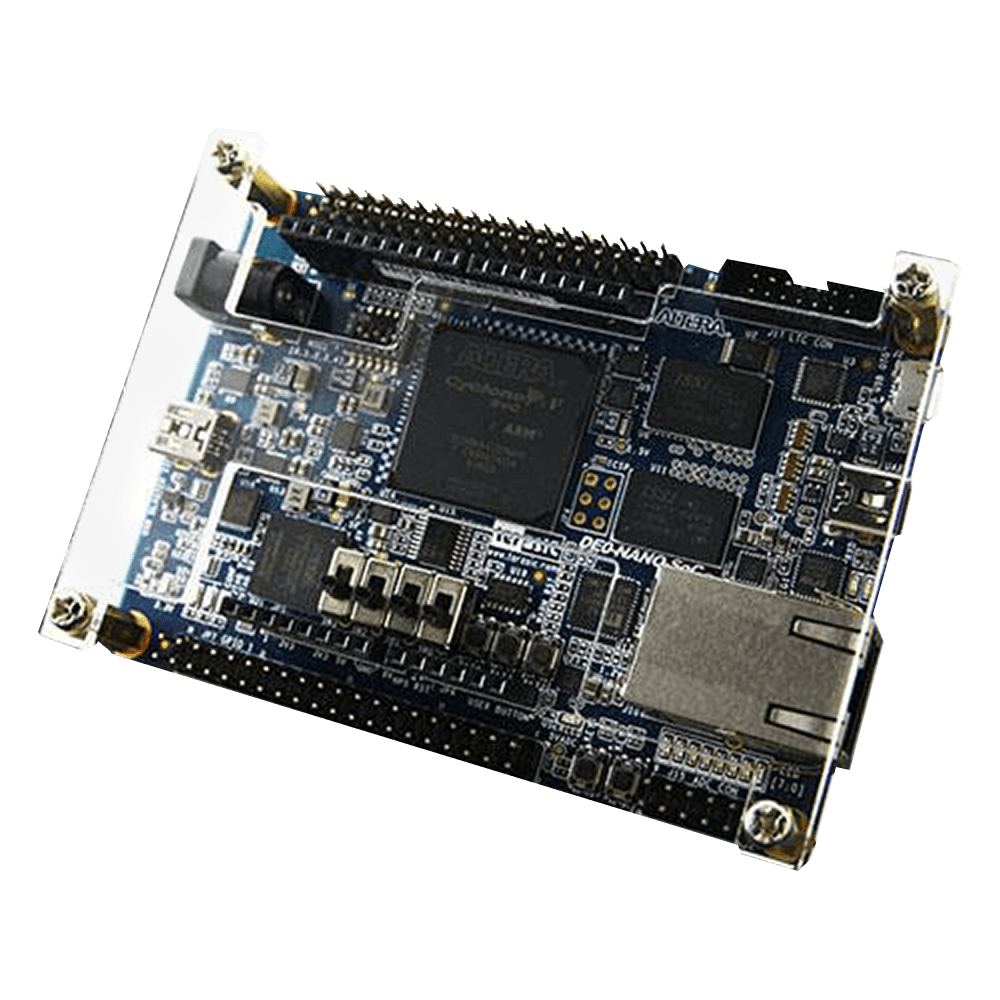
\includegraphics[scale=0.2]{de0-nano-soc.png}}
%     \caption{Układ DE0-Nano-SoC (Cyclone V)}
%     \label{fig:de0-nano-soc}
% \end{figure}




















\chapter{Wstęp}
\label{cha:wstęp}

\section{Wprowadzenie do przetwarzania sygnałów na FPGA}
\label{sec:wprowadzenie}

\subsection{Równoległe przetwarzanie danych}
Współczesne algorytmy cyfrowego przetwarzania sygnałów (DSP) stawiają coraz wyższe wymagania wobec wydajności systemów obliczeniowych.
Tradycyjne procesory, choć rozwijają się pod względem mocy obliczeniowej, napotykają ograniczenia wynikające z sekwencyjnego przetwarzania,
co sprawia, że są mniej efektywne przy obliczeniach, które można prowadzić równolegle. W tym kontekście układy FPGA (Field-Programmable Gate Arrays) wyróżniają się
możliwością równoległego przetwarzania danych, co pozwala na znaczne przyspieszenie złożonych operacji. Dzięki takiemu rozwiązaniu można przetwarzać wiele
strumieni danych jednocześnie, co daje wyraźną przewagę nad klasycznymi procesorami, szczególnie w aplikacjach wymagających wysokiej przepustowości i małych opóźnień.

\subsection{Kontrola zegara i deterministyczne przetwarzanie}
Kolejną zaletą układów FPGA jest możliwość precyzyjnego dostosowania częstotliwości zegara do wymagań projektowych. Dzięki wykorzystaniu języków opisu sprzętu,
takich jak VHDL czy Verilog, projektant ma pełną kontrolę nad wartościami sygałów w każdym takcie zegara, co umożliwia dokładne określenie, kiedy i jakie operacje mają się odbywać.
To daje pewność, że w takich aplikacjach jak filtr FIR dane będą przetwarzane i transmitowane w równych, określonych odstępach czasowych, co jest kluczowe. W odróżnieniu od procesorów,
gdzie prędkość zegara jest sztywno ustalona, a czas wykonywania kodu może być niedeterministyczny -- szczególnie w językach wysokiego poziomu, takich jak Python -- FPGA zapewniają
pełną deterministyczność przetwarzania. Nawet w językach niskiego poziomu użytkownik nie ma pełnej kontroli nad czasem wykonywania kodu, co może prowadzić do pewnych opóźnień.)

\subsection{Platforma Cyclone V SoC}
W mojej pracy skupię się na układzie heterogenicznym firmy Intel -- Cyclone V SoC. Jest to budżetowy układ zawierający w swojej architekturze zarówno FPGA, jak i
HPS (Hard Processor System) oparty na procesorze ARM, co pozwala na rozdzielenie zadań pomiędzy obie architektury. Mimo że Cyclone V SoC nie jest układem najwyższej klasy,
jego cena oraz możliwości konfiguracyjne sprawiają, że znajduje zastosowanie w projektach wymagających kompromisu między wydajnością a kosztami. W mojej pracy pokażę, jak można
efektywnie wykorzystać ten układ do implementacji zaawansowanych algorytmów przetwarzania sygnałów.

\begin{figure}[!htb]
    \centerline{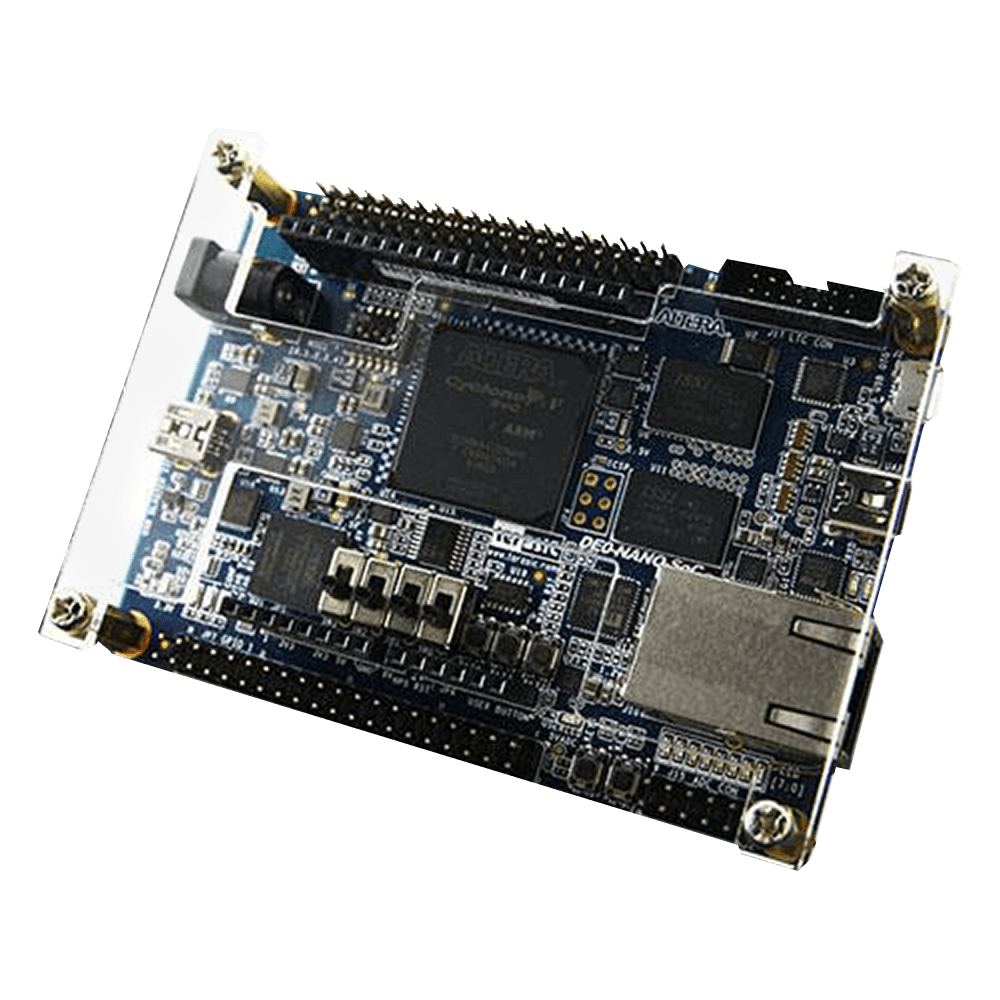
\includegraphics[scale=0.2]{de0-nano-soc.png}}
    \caption{Układ DE0-Nano-SoC (Cyclone V)}
    \label{fig:de0-nano-soc}
\end{figure}

\section{Cele pracy}
\label{sec:celePracy}
Celem pracy jest opracowanie kompleksowego systemu przetwarzania sygnałów. Część FPGA systemu będzie odpowiedzialna za implementację algorytmów DSP, w tym filtru FIR oraz modułu
realizującego dyskretną transformatę Fouriera (DFT). System ten będzie wyposażony w dwie pamięci, pomiędzy którymi dane będą transmitowane, przetwarzane, a następnie zapisywane.

Równocześnie wbudowany procesor będzie pełnił funkcję jednostki sterującej, uruchamiając serwer, który umożliwi użytkownikowi zdalną interakcję z systemem poprzez stronę internetową.
Strona będzie umożliwiać wprowadzanie danych do FPGA, inicjowanie procesów przetwarzania oraz monitorowanie wyników. Taki podział zadań na układ FPGA i HPS umożliwia
efektywną realizację złożonych algorytmów DSP, zapewniając wysoką wydajność oraz intuicyjną obsługę przez użytkownika.




















\chapter{Pierwszy dokument}
\label{cha:pierwszyDokument}

W rozdziale tym przedstawiono podstawowe informacje dotyczące struktury prostych plików \LaTeX a. Omówiono również metody kompilacji plików z zastosowaniem programów \emph{latex} oraz \emph{pdflatex}.

%---------------------------------------------------------------------------

\section{Struktura dokumentu}
\label{sec:strukturaDokumentu}

Plik \LaTeX owy jest plikiem tekstowym, który oprócz tekstu zawiera polecenia formatujące ten tekst (analogicznie do języka HTML). Plik składa się z dwóch części:
\begin{enumerate}%[1)]
\item Preambuły -- określającej klasę dokumentu oraz zawierającej m.in. polecenia dołączającej dodatkowe pakiety;

\item Części głównej -- zawierającej zasadniczą treść dokumentu.
\end{enumerate}


\begin{lstlisting}
\documentclass[a4paper,12pt]{article}      % preambuła
\usepackage[polish]{babel}
\usepackage[utf8]{inputenc}
\usepackage[T1]{fontenc}
\usepackage{times}

\begin{document}                           % część główna

\section{Sztuczne życie}

% treść
% ąśężźćńłóĘŚĄŻŹĆŃÓŁ

\end{document}
\end{lstlisting}

Nie ma żadnych przeciwskazań do tworzenia dokumentów w~\LaTeX u w~języku polskim. Plik źródłowy jest zwykłym plikiem tekstowym i~do jego przygotowania można użyć dowolnego edytora tekstów, a~polskie znaki wprowadzać używając prawego klawisza \texttt{Alt}. Jeżeli po kompilacji dokumentu polskie znaki nie są wyświetlane poprawnie, to na 95\% źle określono sposób kodowania znaków (należy zmienić opcje wykorzystywanych pakietów).


%---------------------------------------------------------------------------

\section{Kompilacja}
\label{sec:kompilacja}


Załóżmy, że przygotowany przez nas dokument zapisany jest w pliku \texttt{test.tex}. Kolejno wykonane poniższe polecenia (pod warunkiem, że w pierwszym przypadku nie wykryto błędów i kompilacja zakończyła się sukcesem) pozwalają uzyskać nasz dokument w formacie pdf:
\begin{lstlisting}
latex test.tex
dvips test.dvi -o test.ps
ps2pdf test.ps
\end{lstlisting}
%
lub za pomocą PDF\LaTeX:
\begin{lstlisting}
pdflatex test.tex
\end{lstlisting}

Przy pierwszej kompilacji po zmiane tekstu, dodaniu nowych etykiet itp., \LaTeX~tworzy sobie spis rozdziałów, obrazków, tabel itp., a dopiero przy następnej kompilacji korzysta z tych informacji.

W pierwszym przypadku rysunki powinny być przygotowane w~formacie eps, a~w~drugim w~formacie pdf. Ponadto, jeżeli używamy polecenia \texttt{pdflatex test.tex} można wstawiać grafikę bitową (np. w formacie jpg).



%---------------------------------------------------------------------------

\section{Narzędzia}
\label{sec:narzedzia}


Do przygotowania pliku źródłowego może zostać wykorzystany dowolny edytor tekstowy. Niektóre edytory, np. GEdit, mają wbudowane moduły ułatwiające składanie tekstów w LaTeXu (kolorowanie składni, skrypty kompilacji, itp.).

Jednym z bardziej znanych środowisk do składania dokumentów  \LaTeX a jest {\em TeXstudio}, oferujące kompletne środowisko pracy. Zobacz: \url{http://www.texstudio.org}


Bardzo dobrym środowiskiem jest również edytor gEdit z wtyczką obsługującą \LaTeX a. Jest to standardowy edytor środowiska Gnome. Po instalacji wtyczki obsługującej \LaTeX~ zamienia się w wygodne i szybkie środowisko pracy.

\textbf{Dla testu łamania stron powtórzenia powyższego tekstu.}


Do przygotowania pliku źródłowego może zostać wykorzystany dowolny edytor tekstowy. Niektóre edytory, np. GEdit, mają wbudowane moduły ułatwiające składanie tekstów w LaTeXu (kolorowanie składni, skrypty kompilacji, itp.).
Jednym z bardziej znanych środowisk do składania dokumentów  \LaTeX a jest {\em TeXstudio}, oferujące kompletne środowisko pracy. Zobacz: \url{http://www.texstudio.org}
Bardzo dobrym środowiskiem jest również edytor gEdit z wtyczką obsługującą \LaTeX a. Jest to standardowy edytor środowiska Gnome. Po instalacji wtyczki obsługującej \LaTeX~ zamienia się w wygodne i szybkie środowisko pracy.
Po instalacji wtyczki obsługującej \LaTeX~ zamienia się w wygodne i szybkie środowisko pracy.

Do przygotowania pliku źródłowego może zostać wykorzystany dowolny edytor tekstowy. Niektóre edytory, np. GEdit, mają wbudowane moduły ułatwiające składanie tekstów w LaTeXu (kolorowanie składni, skrypty kompilacji, itp. itd. itp.).
Jednym z bardziej znanych środowisk do składania dokumentów  \LaTeX a jest {\em TeXstudio}, oferujące kompletne środowisko pracy. Zobacz: \url{http://www.texstudio.org}
Bardzo dobrym środowiskiem jest również edytor gEdit z wtyczką obsługującą \LaTeX a. Jest to standardowy edytor środowiska Gnome. Po instalacji wtyczki obsługującej \LaTeX~ zamienia się w wygodne i szybkie środowisko pracy.

Do przygotowania pliku źródłowego może zostać wykorzystany dowolny edytor tekstowy. Niektóre edytory, np. GEdit, mają wbudowane moduły ułatwiające składanie tekstów w LaTeXu (kolorowanie składni, skrypty kompilacji, itp.).
Jednym z bardziej znanych środowisk do składania dokumentów  \LaTeX a jest {\em TeXstudio}, oferujące kompletne środowisko pracy. Zobacz: \url{http://www.texstudio.org}
Bardzo dobrym środowiskiem jest również edytor gEdit z wtyczką obsługującą \LaTeX a. Jest to standardowy edytor środowiska Gnome. Po instalacji wtyczki obsługującej \LaTeX~ zamienia się w wygodne i szybkie środowisko pracy.

%---------------------------------------------------------------------------

\section{Przygotowanie dokumentu}
\label{sec:przygotowanieDokumentu}

Plik źródłowy \LaTeX a jest zwykłym plikiem tekstowym. Przygotowując plik
źródłowy warto wiedzieć o kilku szczegółach:

\begin{itemize}
\item
Poszczególne słowa oddzielamy spacjami, przy czym ilość spacji nie ma znaczenia.
Po kompilacji wielokrotne spacje i tak będą wyglądały jak pojedyncza spacja.
Aby uzyskać {\em twardą spację}, zamiast znaku spacji należy użyć znaku {\em
tyldy}.

\item
Znakiem końca akapitu jest pusta linia (ilość pusty linii nie ma znaczenia), a
nie znaki przejścia do nowej linii.

\item
\LaTeX~sam formatuje tekst. \textbf{Nie starajmy się go poprawiać}, chyba, że
naprawdę wiemy co robimy.
\end{itemize} 



\chapter{Hardware}
\label{cha:hardware}

\begin{figure}[!htb]
    \centerline{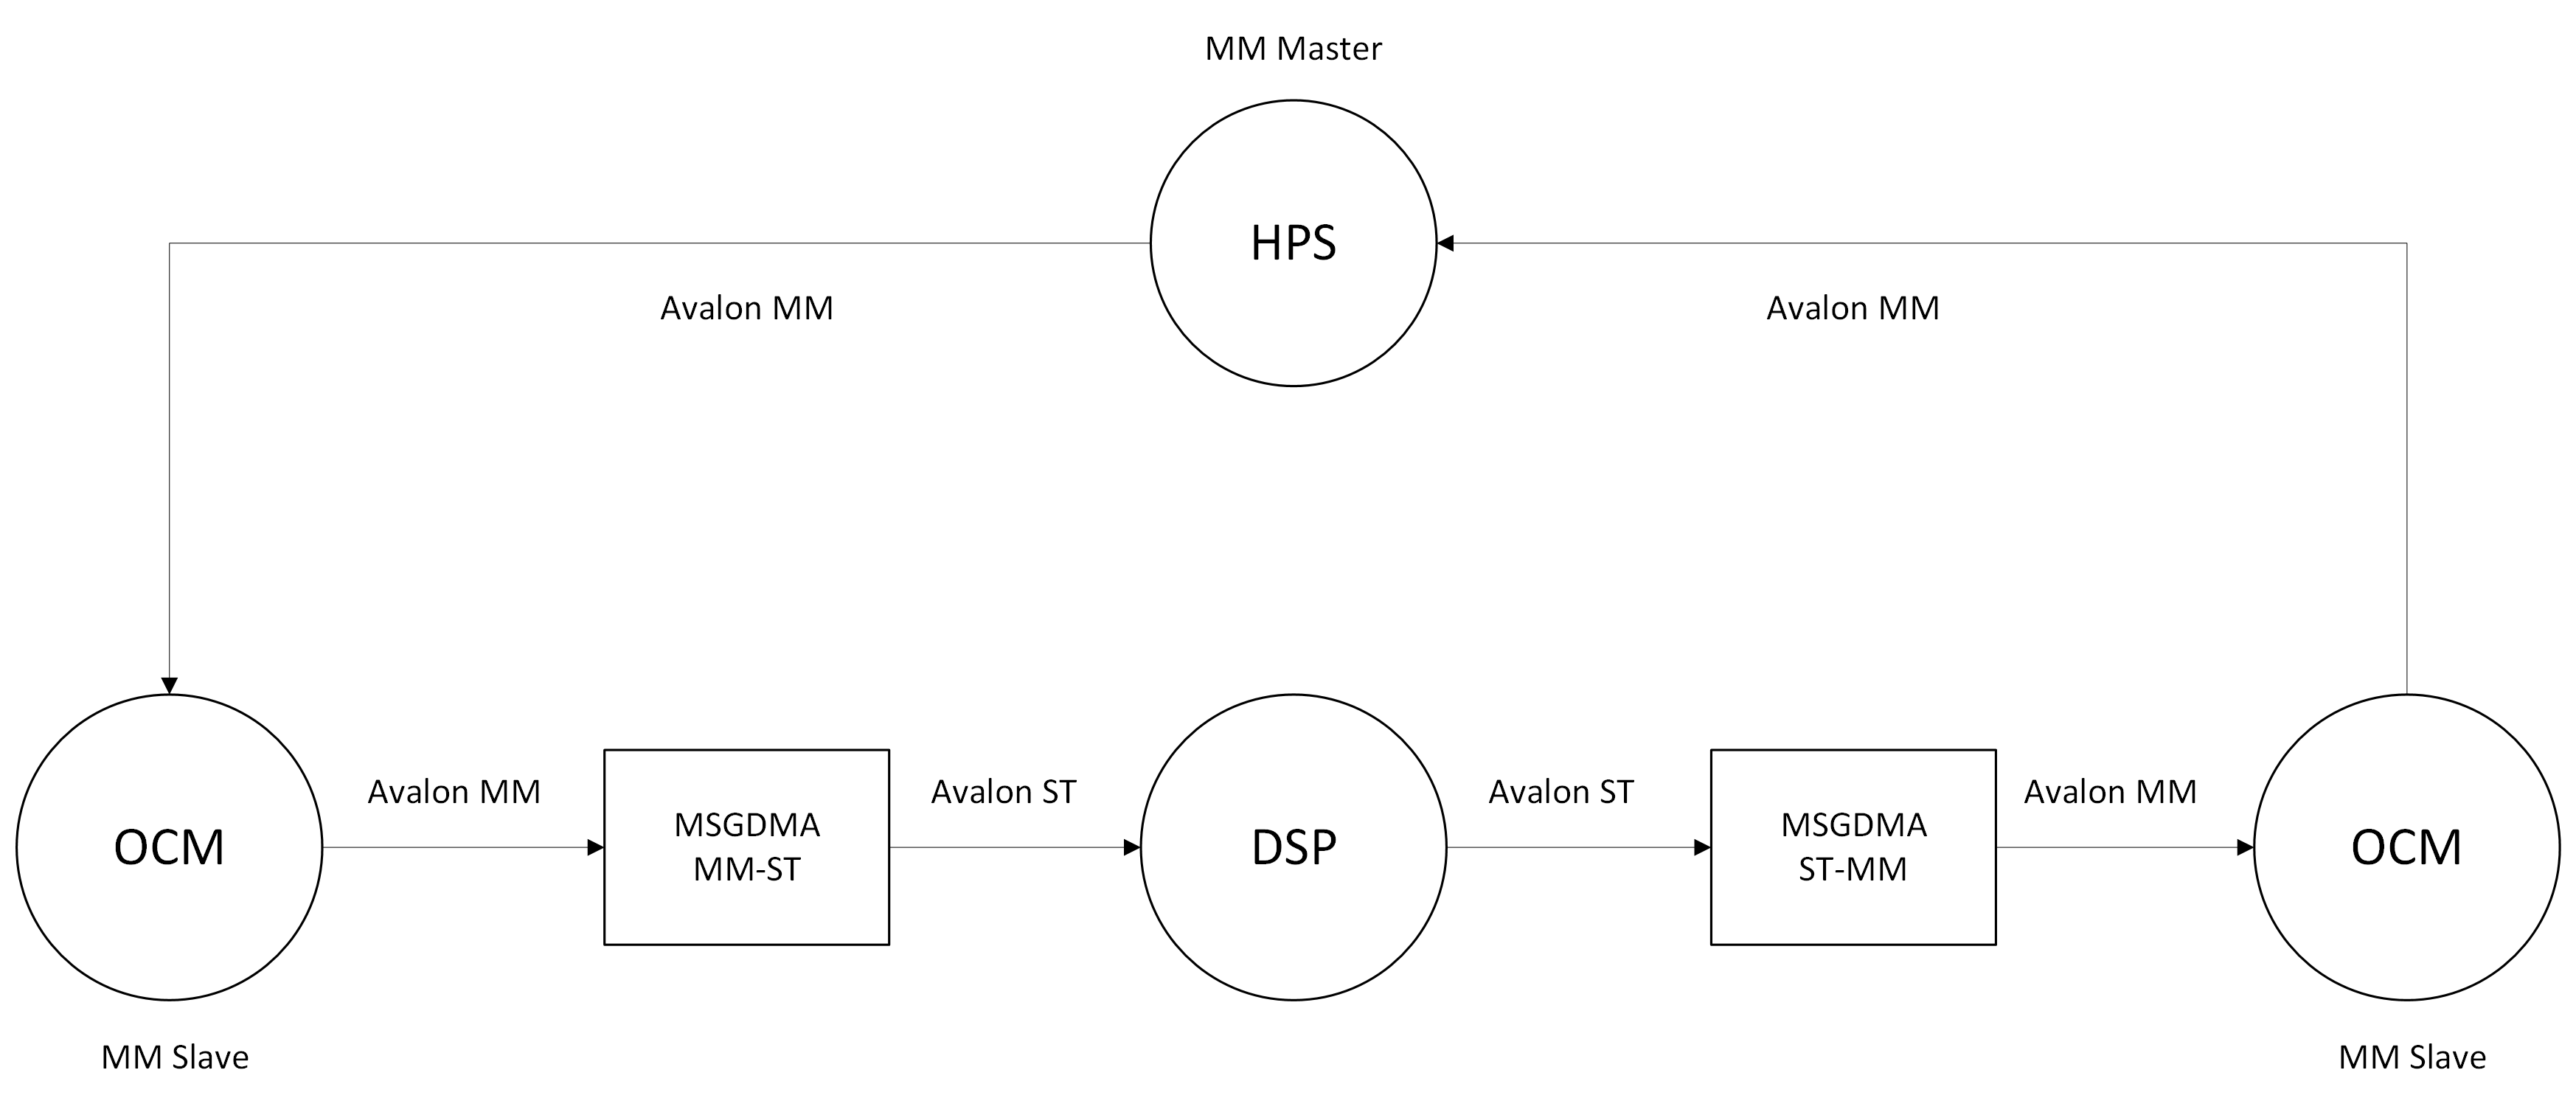
\includegraphics[scale=0.5]{hardwareSystemDiagram.png}}
    \caption{Diagram przedstawiający architekturę sprzętową systemu}
    \label{fig:architektura-hw}
\end{figure}

\chapter{Modular Scatter-Gather DMA}

\section{Avalon MM - Avalon MM}

\begin{table}[h]
    \centering
    \begin{tabular}{|l|p{3.5cm}|p{3.5cm}|p{3.5cm}|}
    \hline
     & \textbf{Szerokość transferu: 32 bity} & \textbf{Szerokość transferu: 64 bity} & \textbf{Szerokość transferu: 128 bitów} \\ \hline
    \textbf{Zegar: 50MHz} & {191.06 MB/s} & {380.63 MB/s} & {720.01 MB/s} \\ \hline
    \textbf{Zegar: 100MHz} & {383.53 MB/s} & {715.43 MB/s} & {1452.71 MB/s} \\ \hline
    \textbf{Zegar: 200MHz} & {724.94 MB/s} & {1480.24 MB/s}  & {2390.95 MB/s} \\ \hline
    \end{tabular}
    \caption{Przepustowość transferu DMA w zależności od częstotliwości zegara i szerokości transferu}
    \label{tab:my_label}
\end{table}


\section{Avalon MM - Avalon ST - Avalon MM}

\begin{table}[h]
    \centering
    \begin{tabular}{|l|p{3.5cm}|p{3.5cm}|p{3.5cm}|}
    \hline
    & \textbf{Szerokość transferu: 32 bity} & \textbf{Szerokość transferu: 64 bity} & \textbf{Szerokość transferu: 128 bitów} \\ \hline
    \textbf{Zegar: 50MHz} & {193.50 MB/s} & {} & {} \\ \hline
    \textbf{Zegar: 100MHz} & {} & {} & {} \\ \hline
    \textbf{Zegar: 200MHz} & {} & {}  & {} \\ \hline
    \end{tabular}
    \caption{Przepustowość transferu DMA w zależności od częstotliwości zegara i szerokości transferu}
    \label{tab:my_label}
\end{table}

% itd.
% \appendix
% \include{dodatekA}
% \include{dodatekB}
% itd.

\printbibliography

\end{document}
